% !TEX root = ../thesis.tex

\chapter{Theory}
\label{chap:theory}

\cleanchapterquote{At the end of the century one will be able to speak of machines thinking without expecting to be contradicted.}{Alan Turing}{(Computing Machinery and Intelligence (1950))}

In this chapter, I cover the basic concepts of Neural Networks that will be used later on when separation of style and content is discussed in more detail.
My intention is to allow anybody with basic knowledge in Mathematics and Computing to understand this manuscript from beginning to end.

The explanations will be developed from basic to complex so that a sequential read should guide the reader logically from question to answer while giving as much insight will be necessary to continue and just enough context to understand the raison d'être of the each concept.


% ------------------------------------------------------------------------------

\section{Background}
\label{sec:theory:background}

Before diving into technical aspects, however, I believe it is worth stopping to first introduce the fields of this thesis: \emph{Neural Networks} and \emph{Deep Learning}.
Neural Networks is an area of \emph{Machine Learning} very closely related with \emph{Cognitive Sciences} and Deep Learning is also an area of Machine Learning that typically uses neural networks, but let us go step by step.


\subsection{Neural Networks}
\label{sub:theory:background:neural-networks}

We can describe the field of Machine Learning as the study that enables computers to resolve problems for which they have not been explicitly programmed for by using some learning mechanism \citet{Samuel1959}.
When explicitly programming an algorithm to resolve a problem its complexity grows dramatically with that of the problem and the desired precision.
A perfectly robust algorithm that follows this approach will require: 1) the programmer to understand the problem completely so that all variables can be taken into account; 2) a hardware powerful enough to handle all these variables; and 3) data with maximum precision.
It is easy to see how one or more of these requirements will pose complications when the problem is complex enough.
Driving a car is a complex enough problem to make Classic Computing incapable of solving it.
Conversely, driving a car is a simple enough problem so that any person can do it.
The human mind can handle the task because, although not having perfect senses nor 100\% understanding of the laws of physics, how the car works, how other drivers exactly behave and many other factors involved; is capable of dealing with partial information, uncertainty, imprecision, and approximations after having learned from experience \cite{Zadeh1994}.
Opposed to how Classic Computing tries to accurately model the world to solve problems, some fields of Machine Learning try to model how the human mind learns the complexity of the world to reason and act upon it.

At this point, it is clear how the study of the human mind plays an important role in Machine Learning.
Cognitive Sciences is the field that studies the human mind and how it acquires understanding through experience and the senses.
Modern Cognitive Sciences have their inception in the 1940s when efforts were being made to understand the principles of the mind by representing their structures and processes instead of operating directly on them \cite{Thagard2008}.
The studies quickly branched off in 1943 when \citet{McCulloch1943}, inspired by biological neural networks, described the first mathematical model of an artificial neural network.
The field Neural Networks, shorthand for \emph{Artificial Neural Networks} (ANNs), quickly grew in the 1950s when they started being implemented \cite{Farley1954,Rosenblatt1958} as approximation or binary classification methods.

Since then, the field has evolved and expanded into a myriad of different methods that have maintained the purity with their biological counterparts in greater or lesser degree.
Within the general framework, we can still talk of neurons organized in \emph{layers}, implementing an \emph{activation function} and storing experience in \emph{weights} as depicted in Figure~\ref{fig:sec:theory:neurons}.
An artificial neuron is a simple processing unit, forming networks typically organized in layers, whose input is the set of outputs of connected neurons from the previous layer and the process it performs is determined by the activation function.
The activation function can be implemented either as a threshold to be reached for the neuron to send an output or simply as a transformation of any sort of the input.
Lastly, experience in ANNs can be understood as connection strength between neurons in biological neural networks and this mechanism is implemented as a set of learnable parameters, commonly called weights, that modifies the value of each input of the neuron \cite{Hinton1990}.

\begin{figure}[htb]
  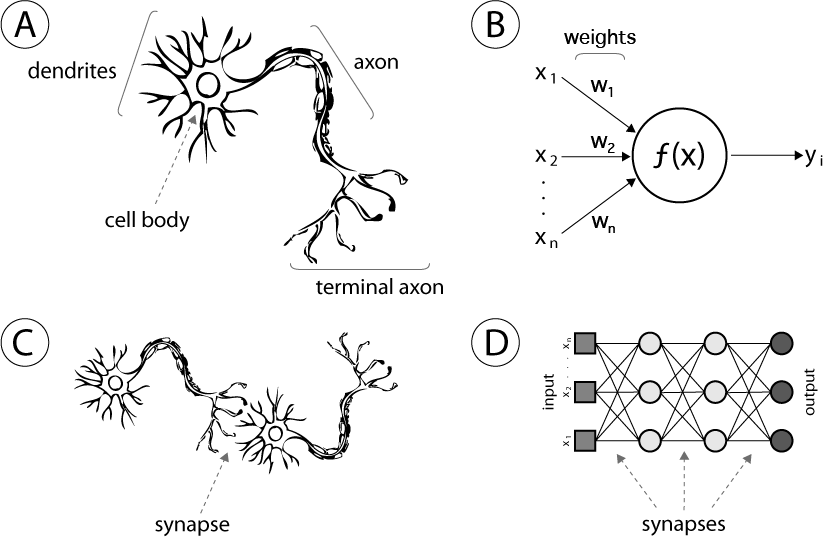
\includegraphics[width=\textwidth]{gfx/neurons}
  \caption{Biological Neuron vs Artificial Neuron \cite{Honorio2013}.
    AC) A biological neuron receives signals at the dendrites, the composition of the signals may or may not produce an excitation in the cell body based on experience, in which case a pulse will be transmitted down the axon and ultimately to other neurons' dendrites via terminal axon in a process called synapsis.
    BD) Similarly, artificial neuronal networks are organized in layers and synapsis occurs from layer to layer.
    An artificial neuron in the layer $Y$ receives one or more inputs $X$, representing dendrites, and as a result of an activation function $f(X)$ produces an output $y_i$, representing the axon, that gets passed to connected neurons in the subsequent layer.
    Weights represent connection strength between neurons and encode network experience.}
  \label{fig:sec:theory:neurons}
\end{figure}

A crucial step in preparing an ANN for a specific task is refining its set of weights.
That is what we refer to as training or supervised learning process.
Supervised learning is a data-driven process that requires a labeled training set of examples of which we know their class (dog vs. cat).
The process can be implemented in several ways but it generally boils down to defining some way to assess how far the prediction of the network is away from an optimal solution, known as the \emph{loss function}, and the strategy that will propagate the error to refine the weights of the network.
Eventually, after enough training examples and corrections, the weights of the network will have adapted to generalize the features of the training data and will be more or less able to correctly classify new incoming examples.

The process can be seen as a teacher supervising the learning of a student.
The ``teacher" (loss function + weight rectification strategy) knows the correct solution (label of the example) and it corrects the ``student" (the network) when its prediction is incorrect.
An example of a completely wrong prediction would be the network having 100\% confidence of an image containing a dog when it clearly contains a cat.

One of the most important aspects that determine the accuracy of the network when presented with new examples is the volume of data and the correctness of its labels.
This becomes extremely important when trying to solve real-world problems like image recognition, where massive training sets are required to generalize networks for all concepts in a language under several different lighting conditions.
Big enough volumes of data have not been available until recently, and even nowadays, complete and accurately labeled datasets are expensive or time consuming to handcraft as the task may be too large or require expert knowledge on the specific field.
Approaches to work around this involved using partially labeled training datasets and pre-training the network first with unsupervised training where unlabeled examples with similar features are grouped together, then classified after the learning phase and finally used as additional training data \cite{Hinton2006}.
This approach is called semi-supervised learning and is one of the achievements of Deep Learning, which I am discussing next.


\subsection{Deep Learning}
\label{sub:theory:background:deep-learning}

Since 2006 the field of \emph{Deep Learning}, also called hierarchical learning, has appeared as a new area of Machine Learning research that brings it closer to its original goals: Artificial Intelligence \cite{Deng2014}.
Deep Learning focuses its efforts on producing methods for learning hierarchical feature representations, different levels of abstraction where higher-level ones are defined from lower-level ones, helping to make sense of data such as images, sound, and text in real-world applications.

One clear example of hierarchical representation is a spoken sentence.
A spoken sentence, the higher-level concept, is composed of spoken words.
A spoken word is made up of phonemes.
A phoneme is a representation of a speech sound with an associated waveform.
Making sense of speech in Deep Learning means first analyzing the waveform looking for phonemes, then trying to make up words from the phonemes found, and finally producing a grammatically correct and semantically meaningful sentence with those words.

As already mentioned in chapter~\ref{chap:intro}, this kind of pattern recognition did not perform well until recently.
Traditional solutions employed shallow neural networks with simplistic models and limited representation power that could only be used to solve well-constrained problems like numerical approximations or binary classification.
Speech recognition, contrarily, is a very loosely-constrained problem and that is also the case for any problem dealing with the richness of data such as human voice, natural language, and natural images.

Studies in human information processing mechanisms suggested the human brain uses deep neuronal architectures to extract complex patterns and build internal representations from rich sensory inputs.
For instance, the human speech perception system in the brain is equipped with layered hierarchical structures that transform the information from the acoustic level to the linguistic level \cite{Deng1999,Baker2009}.
Training analogous deep architectures in artificial neural networks, \emph{deep neural networks} (DNNs), proved problematic from the beginning since classic learning algorithms tended to easily get trapped in poor local optima parameters.
This phenomenon, unfortunately, worsened quickly the more layers the neural network presented, which is the case of DNNs.

Efficient unsupervised learning algorithms that made use of the increasingly big datasets, available thanks to the widespread use of the Internet, were proposed to overcome the problems presented by local optima in classic learning algorithms \cite{LeCun2004,Hinton2006}, as previously discussed in Section~\ref{sub:theory:background:neural-networks}.
They, however, were so computationally expensive for training deep neural networks, having millions of parameters to learn, that were not widely used until parallelizable variations were proposed in 2012 \cite{Dean2012,Chen2012}.
These, alongside with powerful Graphic Processing Units (GPUs) becoming a commodity enabling the implementation of these algorithms marked the rapid expansion of Deep Learning in recent years.

Deep Learning is at the moment a quickly growing field covering a wide range of Machine Learning techniques and architectures.
In this thesis, I cover only the architecture of DNNs that we need for further discussing the separation of style and content, \emph{Convolutional Neural Networks} in Section~\ref{sec:theory:convnets}.
Before jumping too far ahead, the next sections of this chapter will go through the evolution of relevant ANNs architectures down from the most basic one, the \emph{perceptron}, up to the one at hand, Convolutional Neural Network.


% ------------------------------------------------------------------------------

\section{Perceptron}
\label{sec:theory:perceptron}

The perceptron was the first ever implemented neural network.
It was created by \citet{Rosenblatt1958} in 1957 based on the studies of \citet{McCulloch1943} and it featured the simplest architecture possible in an ANN, composed of a single neuron.

The perceptron can be described as performing a task of binary classification, which is simply deciding in which of two mutually exclusive classes a set of inputs belongs \cite{Freund1999} and it is mathematically expressed as follows:

$$
  f(x) =
  \begin{cases}
    1 & \text{if } {w}\cdot{x}+b > 0\\
    0 & \text{otherwise}
  \end{cases}
$$

Where $x$, an array of real values, represents the input of the perceptron; $w$, also an array of real values, represents the weights; $b$ is the \emph{bias}; ${w}\cdot{x}$ is the dot product; ${w}\cdot{x}+b > 0$ is the activation function; and $0$ and $1$ are the representation of the mutually exclusive classes.

The inputs are visualized as data points in the space of variables and the activation function as a linear boundary that leaves them classified either above or below it.
The weights are used to measure the relevance of each one of the inputs in the final classification, parameters that get learned during the training process in the same fashion as I described in Section~\ref{sub:theory:background:neural-networks}.
The bias gets also learned during the training process, but it does not depend on any input value and is used to control the position of the linear boundary.
The dot product can also be expressed as a weighted sum $\sum_{i=0}^{m} w_i x_i$ where $m$ is the number of parameters the perceptron receives per input, as it is depicted in Figure~\ref{fig:sec:theory:perceptron}.

\begin{figure}[htb]
  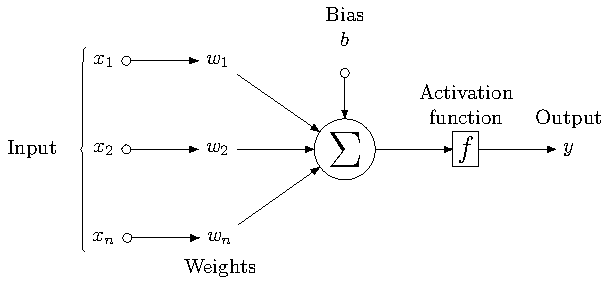
\includegraphics[width=\textwidth]{tkz/perceptron}
  \caption{Anatomy of the Perceptron \cite{Medina2013}.
    In the center, represented by $\sum$, there is the weighted sum of inputs.
    Mathematically expressed as the dot product (${w}\cdot{x}$) of the vector of inputs $x$ with the vector of weights $w$, both containing real values.
    The activation function triggers a binary output $y$ if ${w}\cdot{x}$ plus the bias $b$, also a real value, is above $0$.}
  \label{fig:sec:theory:perceptron}
\end{figure}

Perceptrons can be trained with supervised learning for trying to find the weights in the binary classifier function to correctly classify some training dataset.
Let us imagine we want to train a perceptron to classify animals into either cat or dog based on their size and level of domestication.
Our training data is labeled, meaning that for each pair $(size, domestication)$ we know whom it actually belongs to, either a cat or a dog.
We start with a perceptron whose weights are set to random values and the first training example gets classified randomly.
As new training examples arrive, the learning algorithm will update the weights of the perceptron so that the linear boundary described by ${w}\cdot{x}+b$, the activation function, leaves data points correctly classified in both sides.
Figure~\ref{fig:sec:theory:perceptron-training} depicts how this process happens.

\begin{figure}[htb]
  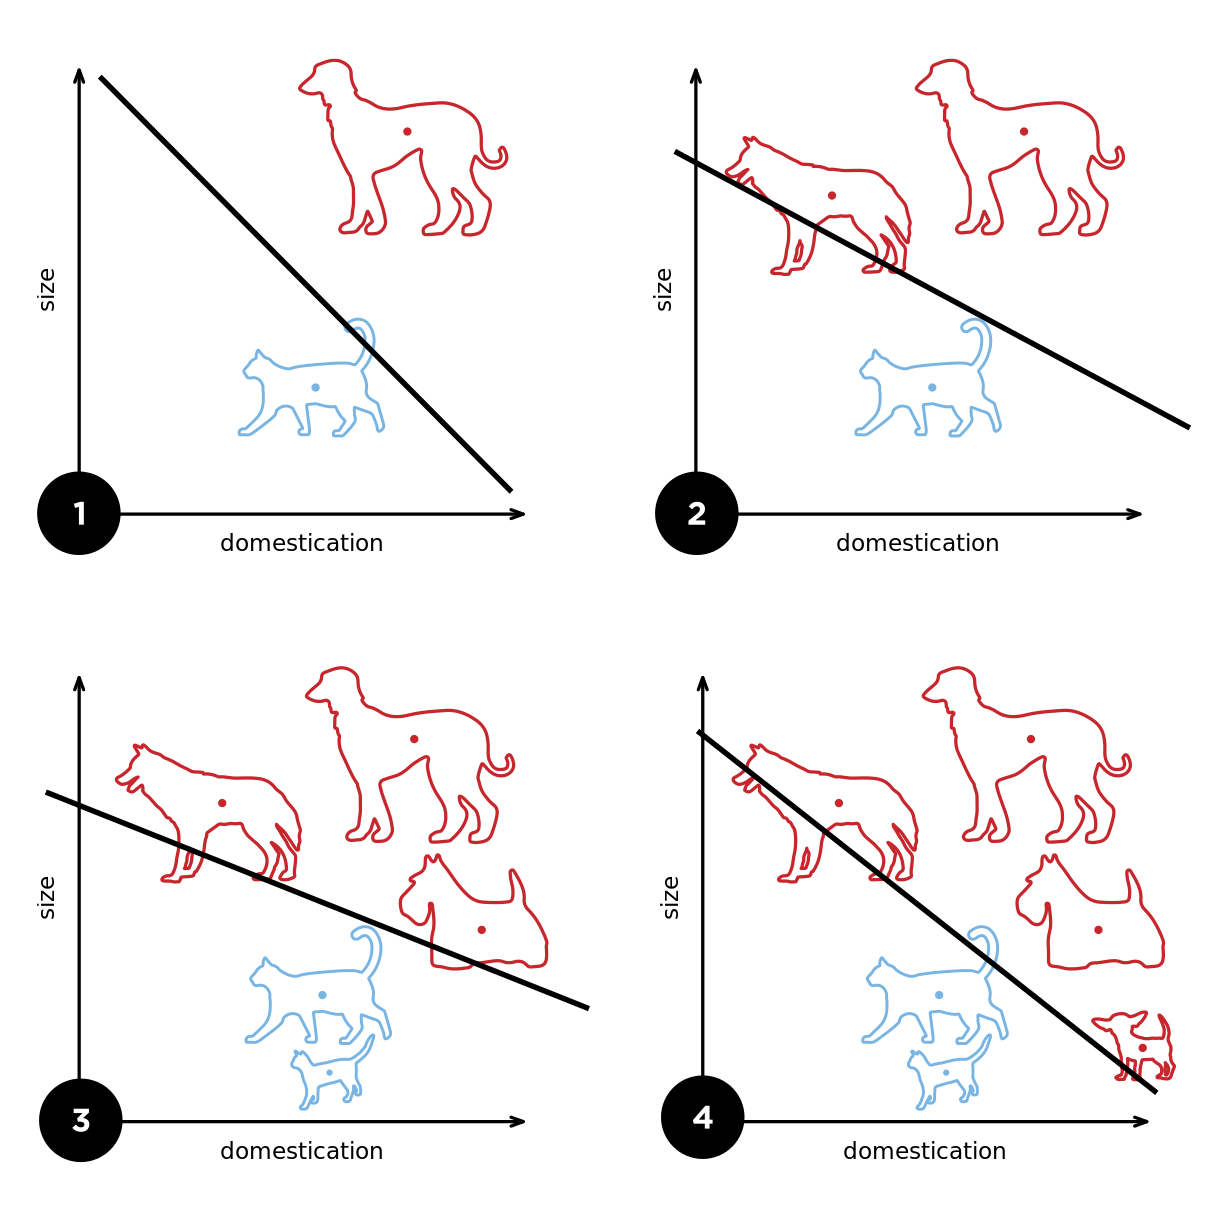
\includegraphics[width=\textwidth]{gfx/perceptron-training}
  \caption{Linear boundary of a perceptron adjusting to new training examples \cite{Goodspeed2015}.
    The perceptron classifies inputs with two variables: $size$ and $domestication$, into two classes, dog or cat.
    Supervised learning adjusts the linear boundary to accommodate the new data points into their correct category.}
  \label{fig:sec:theory:perceptron-training}
\end{figure}

The main problem with the perceptron is that the training will never converge to a set of weights that correctly classify the training examples if these are not linearly separable, and thus predictions of new data points will consistently be wrong.
These limitations were mathematically proved by \citet{Minsky1969} in 1969.
Not only that, they also claimed perceptrons with multiple layers of neurons would not be capable of overcoming non-linearities, leading to believe that Neural Networks would not be feasible for scalable intelligent systems and managing to discourage further efforts in the field for over a decade.
Little to none research was done in Neural Networks until \emph{backpropagation}, a learning algorithm for \emph{multilayer perceptrons}, was developed by \citet{Werbos1974}, rediscovered by \citet{Parker1985}, and finally popularized by \citet{Rumelhart1988} in 1988 \cite{Ruck1990}.
The multilayer perceptron marked the comeback of Neural Networks and is the previous step before being able to talk about Convolutional Neural Networks.


% ------------------------------------------------------------------------------

\section{Multilayer Perceptron}
\label{sec:theory:mlp}

While discussing the perceptron, we could not really speak of it as neural network per se, since it consists of a single neuron.
A multilayer perceptron (MLP), however, is a neural network with multiple layers of neurons, them being fully connected with the neurons of the next layer.
Figure~\ref{fig:sec:theory:mlp} depicts the architecture of a simple MLP, where data, represented as arrows, always flows forward and the network does not present any cycle.
This type of architecture is referred to as \emph{feed-forward}, opposed to other more complicated types of architectures where data is fed back to previous layers.
In MLP, the first layer represents the parameters of the input, in the same fashion as we saw for the perceptron.
The final layer performs the classification, also like the perceptron.
Intermediate layers, called \emph{hidden layers}, are the most interesting addition to the architecture.
Neurons in them perform intermediate predictions and these are fed to neurons in the next layer.
MLP's architecture allows for different neurons in the hidden layers to make predictions of different patterns in the raw input and letting neurons of subsequent layers predict based on patterns instead.

\begin{figure}[htb]
  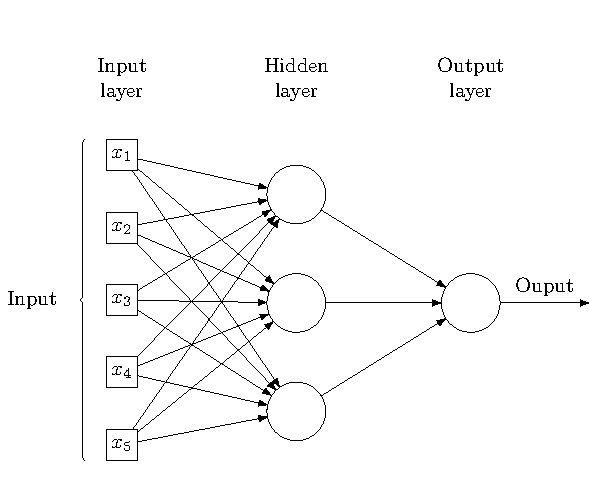
\includegraphics[width=\textwidth]{tkz/mlp}
  \caption{Architecture of the most simple multilayer perceptron \cite{Medina2013A}.
  The first layer, at the left, represents the parameters of the input that get fed into each one of the neurons of the next layer.
  The last layer, at the right, performs the final classification.
  The layers in between, called hidden layers, also perform intermediate classification and their output is fed as input to the next layer.}
  \label{fig:sec:theory:mlp}
\end{figure}

If we zoomed in on one the nodes we would see replicated exactly the same structure as in the perceptron from \autoref{sec:theory:perceptron} (\autoref{fig:sec:theory:perceptron}).
Inputs get weighted and summed, and the result of that passed to some function that performs the prediction.
One important difference to note is that for the input of subsequent layers to still be real values, neurons in hidden layers must implement non-linear activation functions, representing the probability or certainty of the example belonging to a class.
Non-linear activation functions are also normally called \emph{transformation functions} since they transform the input rather than producing a binary classification.
Non-linearities often used are the hyperbolic tangent, $\tanh(x)$, or the logistic function, $(1+e^{-x})^{-1}$, which are inspired by biological neurons' \emph{action potential}, and allow for non-linear classification \cite{Thorpe1989}.

Knowing MLP neurons in the output layer behave exactly the same as the perceptron, we can redefine it as a special case of MLP with a single layer and a single neuron on it, often called \emph{single-layer perceptron}.
Unlike single-layer perceptron and contrary to \citeauthor{Minsky1969}'s belief, disproved by \citet{Hornik1989} in 1989, MLPs with at least one hidden layer are capable of making predictions of arbitrary precision given enough data regardless of it being non-linearly separable.
MLPs' capabilities make of them universal approximators and viable for intelligent systems, being the key for such an achievement backpropagation, a general purpose supervised learning algorithm for feed-forward networks \cite{Rumelhart1986}.


\subsection{Backpropagation}
\label{sec:theory:mlp:backpropagation}

Training single-layer networks, where the input is directly connected to the output layer, is relatively simple.
As we saw for the perceptron, it only requires iteratively adjusting the weights to correctly classify the training examples based solely on the input parameters.
Training multi-layered networks becomes much more difficult since the final prediction is not directly related to the original input parameters, but to all intermediate predictions in hidden layers and thus to their weights as well.
Consequently, a learning procedure for MLPs should determine the weights of neurons in hidden layers that will result in the intermediate predictions that will produce correct predictions at the output of the network.
This is equivalent to making the neurons in hidden layers learn internal representations of incoming data, which is one of the main interests of using multi-layered networks to solve real-world problems that are hard to model, be it due to lack of knowledge in the domain or to the complexity of the task.

Learning in neural networks can be generally approached as an optimization problem.
For each training example $(x, t)$, being $x$ the array of input parameters, we first must find the minima in the error function $E = (t - y)^2$, being $t$ the correct prediction, also referred to \emph{ground truth}, and $y$ the prediction of the network.
At the same time, $y$ is a function representing the operation performed by the network as a whole, depending on the weights $w$ that will ultimately be adjusted to minimize the error $E$.

\autoref{fig:sec:theory:mlp:error-function} shows the visual representation of the error function for a single-layer perceptron with 2-parameter inputs, being $y = w_1 x_1 + w_2 x_2$, the transformation function.
There are several methods to find the minima of such parabolic function, but \emph{gradient descent} is normally used.
In multi-layered networks, on the other hand, $y$ is a composite function of increasingly nested transformation functions on each layer.
For an MLP $y$ would be $\sum_i w_i f_i(x)$, being $i$ neurons of the last hidden layer, $w_i$ the weight assigned to their output, and $f_i$ their transformation function, described by $\sum_j w_j f_j(x)$, being $j$ neurons of the previous hidden layer.
This continues until the first hidden layer.
Gradient descent can be efficiently applied on this kind of chained functions using the chain rule, as described by \citet{Linnainmaa1976} and implemented in Backpropagation.

\begin{figure}[htb]
  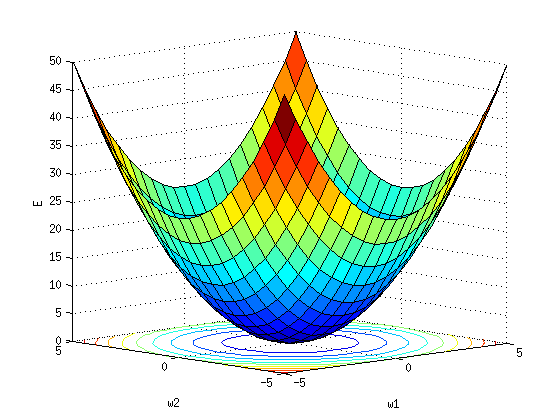
\includegraphics[width=\textwidth]{gfx/error-function}
  \caption{Error function of a single-layer perceptron with two input weights \cite{AI4562013}.
    The function is defined by $E = (t - (w_1 x_1 + w_2 x_2))^2$ and finds its minima at $E = 0$ when $w_1$ and $w_2$ correctly predict $t$ for the input $x$.}
  \label{fig:sec:theory:mlp:error-function}
\end{figure}

Backpropagation, inspired on the mathematical intuition, describes an approach for adjusting the weights of the whole network based only on the output prediction error and capable of scaling up for arbitrarily big networks by propagating the error and correcting weights locally for each neuron.
The algorithm consists of two phases: 1) error propagation, and 2) weight correction.

In error propagation, for a training example, the algorithm first calculates the error $E$ for the prediction $y$ in the output layer.
The error gets then propagated backwardly to all neurons layer by layer, as represented in \autoref{fig:sec:theory:mlp:backprop-1}.
The propagated error for a neuron $i$ within a given hidden layer is calculated as $E_{i} = \sum_j w_{ij} E_{j}$, being $j$ a neuron in the following layer (closer to output), $E_{j}$ its calculated error, and $w_{ij}$ its associated weight for neuron $i$.
Propagated errors represent how much of the overall error was contributed by the neuron on its layer.

Once the error has been calculated for the first hidden layer, the weight correction phase begins.
Starting from the first hidden layer, each weight of every neuron is adjusted by finding the optimal value that minimizes the error for that neuron using the original input $x$.
Once all weights of a layer are adjusted, the neuron outputs, now updated due to having adjusted weights, are used as input to optimize weights of subsequent layers, as depicted in \autoref{fig:sec:theory:mlp:backprop-2}.
This is done by applying gradient descent, which is achieved by \todo{don't fully understood}{calculating the partial derivative of the error with respect to a given weight}.

$$\Delta w_i = \frac{\partial E}{\partial w_i} = E \frac{df(x)}{dx}x_i$$

\begin{figure}[htb]
  \begin{subfigure}[b]{0.5\textwidth}
    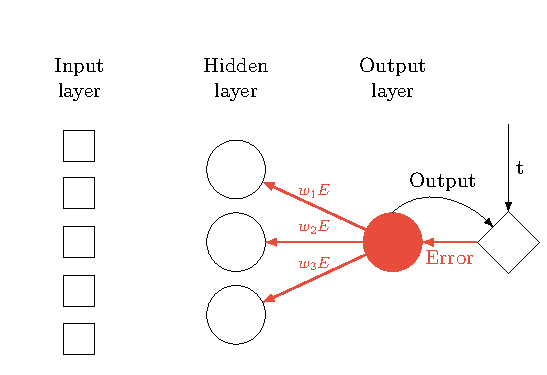
\includegraphics[width=\textwidth]{tkz/mlp-backpropagation-1}
    \captionsetup{justification=centering}
    \caption{Error propagation}
    \label{fig:sec:theory:mlp:backprop-1}
  \end{subfigure}
  \hfill
  \begin{subfigure}[b]{0.5\textwidth}
    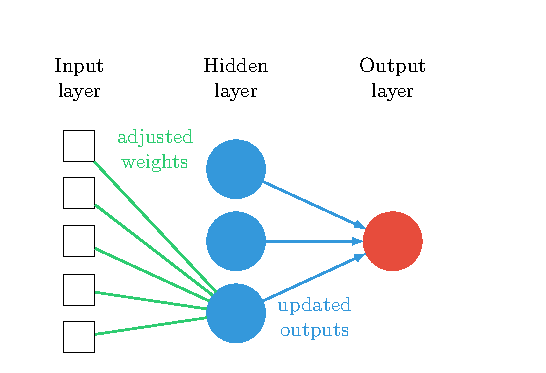
\includegraphics[width=\textwidth]{tkz/mlp-backpropagation-2}
    \captionsetup{justification=centering}
    \caption{Weight correction}
    \label{fig:sec:theory:mlp:backprop-2}
  \end{subfigure}
  \caption{Backpropagation.
    In error propagation (a), the error $E$, calculated as $t - output$, is propagated from the output layer to all hidden layers, representing how much each neuron contributed to the overall error.
    In weight correction (b), having the propagated error for all neurons and starting by the first hidden layer, gradient descent can be applied to optimize each weight for every neuron receiving the original input.
    After all weights in a layer are adjusted gradient descent is applied in the subsequent layers using the updated outputs.}
  \label{fig:sec:theory:mlp:backprop}
\end{figure}

\todo[inline]{maybe talk about the learning rate?}

% There is usually a learning rate parameter that makes gradient descent not to override the weights but simply shift them towards or away from the optimal value for that particular training example.
% This parameter must be carefully chosen to make the training process converge and \todo{is that so?}{avoid overfitting}.

For a more in-depth step by step explanation of backpropagation, I recommend further reading \url{http://home.agh.edu.pl/~vlsi/AI/backp_t_en/backprop.html} \cite{Bernacki2005}.

There is still one final concern when training MLP.
Backpropagation trains MLP to accurately predict samples from the training dataset, but the ultimate goal of training a neural network, we must not forget, is making it capable of predicting unseen samples.
We, therefore, evaluate the performance of a trained network based on how accurate it predicts unseen samples, and when it fails at the task after the learning process we say it is \emph{overfitted}.


\subsection{Overfitting}
\label{sec:theory:mlp:overfitting}

We refer to overfitting when a trained neural network has excellent accuracy against samples in the training dataset, but low accuracy against unseen samples.
Overfitting may occur mainly because of two reasons: 1) not having enough training samples to train the network, 2) the training dataset being too noisy.

When there are fewer learnable parameters than training samples the network will simply ``memorize'' how to match training samples to correct predictions.
If more training samples are given than $input \rightarrow prediction$ associations the network can ``memorize'', it will be forced to learn patterns instead.
For instance, going back to the example of classifying animals as either cat or dog we used in \autoref{sec:theory:perceptron}, if we only had two training samples: a cat, small and wild; and a dog, big and docile; the network would wrongly assume all small animals are cats and a chihuahua would end up classified as a feline.

The training dataset is noisy when training samples contain parameters weakly correlated with the prediction task.
Returning once more to cat and dog classification, if we added the birth date to the dataset we would be increasing the noise.
We know birth date is hardly correlated with an animal being a cat or a dog, but if by any chance all cats in the training dataset got born in 2015 and all dogs in 2016, the network would probably fail its prediction when presented with a kitten born in 2016 because it learned that getting born in 2016 was a feature only present in dogs.
Another case of noise would be the dataset containing extreme cases, like some very domesticated circus tigers.
Training the network with a few of them will be useful for classifying unseen circus tigers as cats, however, if the training process prolongs the network may end up classifying big domestic dogs also as cats.

Dealing with overfitting is not a trivial matter, especially when training big networks for real-world applications.
Big networks with too many learnable parameters are more sensitive to noise and end up picking up lots of uncorrelated parameters that are less obvious than in the previous examples.
Preparation of training datasets for training effective networks becomes crucial, but it is generally hard to decide what is noise and what is valuable data in many cases.
On top of it, learnable parameters increase exponentially when input data is rich and when the network has multiple layers, and because of this, vast amounts of training data are required, making the dataset preparation process even more laborious.

Although MLPs are universal approximators, their fully connected architecture makes them extremely prone to overfitting, as the number of learnable parameters quickly grow with every neuron added to the network.
Overfitting made MLPs outperformed by domain specific algorithms, relegating neural networks to a secondary position in many areas of Machine Learning for some time.
In tasks like image or speech recognition, MLPs suffered terribly the effects of overfitting to the point of not being truly usable, displaying frustrating performance when used in end-user applications as I illustrated in chapter~\ref{chap:intro}.

I will next discuss how Convolutional Neural Networks, developed in the late 90s, eventually proposed a feed-forward multilayer architecture capable of performing robustly image and speech recognition, among others tasks.
They require far fewer learnable parameters than MLPs, avoiding the extreme effects of overfitting seen in MLPs, and are currently state-of-the-art in many pattern recognition tasks.


% ------------------------------------------------------------------------------

\section{Convolutional Neural Networks}
\label{sec:theory:convnets}
Convolutional Neural Networks, also known as CNNs or ConvNets, are feed-forward multilayer neural networks inspired by cats' and monkeys' visual ventral stream \cite{Hubel1968,Lawrence1997} and are responsible for a major breakthrough in image recognition \cite{LeCun1995}.
Before and contemporaneous to \citeauthor{LeCun1998}'s LeNet \cite{LeCun1998} other networks like \citeauthor{Fukushima1980}'s Neocognitron \cite{Fukushima1980} or \citeauthor{Riesenhuber1999}'s HMAX \cite{Riesenhuber1999} were also inspired in the visual cortex, but it was the former that established the fundamentals for CNNs.
They are able to learn patterns in images from a training set through back-propagation and present built-in resilience towards translation and distortion variances in the input.
Such resilience minimizes pre-processing tasks both for training and classification and greatly reduces human supervision, making CNNs the currently preferred system for image recognition \cite{Visin2015}.

MLP were able to perform image recognition \cite{Zhang1999} but in order to reduce the effects of overfitting they could only perform scope-specific predictions on low-res images that had to be processed beforehand to reduce noise.
Fully connected layers scale poorly since neurons of the first hidden layer will process the whole image and will need to store weights for every color channel of every pixel.
Just to give a sense of the scale we are talking, for an RGB image of ${N}\times{M}$ pixels, every neuron in a multi-layer perceptron will require storing ${N}\times{M}\times{3}$ weights, which for a ${32}\times{32}$ image it is $3072$ weights, but for a ${1024}\times{1024}$ one is more than $3$ million.
This means a quadratic memory growth $O(N^2)$ with respect to image resolution.
Not only this is the cause of huge overfitting effects, it also implies a performance issue in terms of hardware resources.

One big wrong assumption in MLPs, derived from their fully-connected nature, is treating each input parameter individually as non-correlated data.
This is false in tasks of signal processing, speech recognition or image recognition.
For instance, let us image a set of images containing a red apple.
Pixels on it are not randomly distributed but, rather, red-hued pixels are expected to bunch together.
It seems the rule \emph{``bunch of red-hued pixels $\rightarrow$ apple''} should be sufficient to recognize an apple, no matter if the bunch of pixels appears either centered or shifted to one side.
MLPs' pitfall is two-fold here.
On the one hand, the network will probably fail if the apple is shifted too much on one side since it did not just the rule proposed before but more likely: \emph{``pixels in positions $(4, 4)..(4, 6)...(6, 4)..(6, 6)$ are red $\rightarrow$ apple''}.
On the other hand, every neuron ``sees'' the whole image so the rule will be learned in several different sub-networks as some sort of brute-force pattern learning.
This intuition tells us MLPs require a bigger amount of learnable parameters that should be needed and that is, in fact, the cause of overfitting problems.

CNNs can take advantage of spatial information inherent in data thanks to a number of CNN architectural features \cite{LeCun1998}: 1) local receptive fields, 2) shared weights, and 3) subsampling.


\subsection{Properties}
\label{sub:concepts:convnets:properties}

\paragraph{Local receptive fields}
The term \emph{receptive field} is borrowed from the literature of neuroscience and it refers to an area of the body surface that trigger a neurological response in the presence of stimuli \cite{Sherrington1906,Alonso2008}.
In the context of convolution networks, receptive field refers to a region of the visual input, represented by an image, that is connected with one or several neurons that will react to it and is commonly called \emph{filter}.
Using local receptive fields means that neurons in the network will not react to the whole image but to a small region of it instead.
This ensures neurons will extract first the most basic visual features such as edges, end-points or corners;
In subsequent layers, from those elementary visual features, neurons will then extract progressively higher-order features like shapes, textures, faces or objects.
Such architecture allows effectively taking into account the spatial correlation existing in images.
Within a layer, several neurons performing different feature detections can be stacked to receive the input from the perceptive field as depicted in Figure~\ref{fig:sec:theory:convnets:conv-layer-1}.

\begin{figure}[htb]
  \begin{center}
    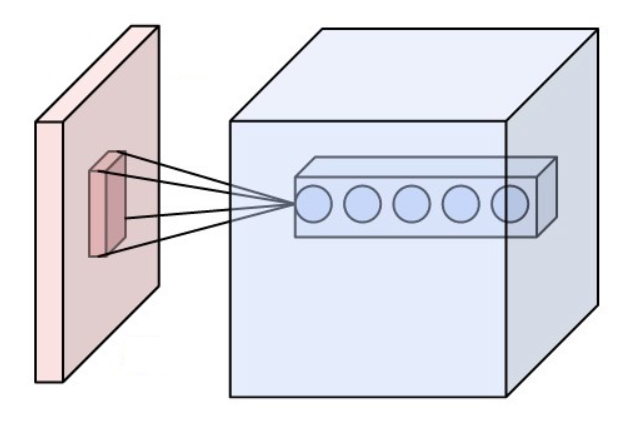
\includegraphics[width=0.6\textwidth]{gfx/conv-layer-1}
  \end{center}
  \caption{Stack of neurons applying different feature detections within a convolutional layer on the same perceptual region \cite{Aphex342015}.}
  \label{fig:sec:theory:convnets:conv-layer-1}
\end{figure}

\paragraph{Shared weights}
Layers in CNNs are organized in several slices, each of them containing neurons that detect the same feature but in different regions of the image and each slice detecting different features.
This operation is equivalent to a convolution in image processing, a sliding window that applies a transformation the original image, and that is where CNNs receive their name.
The sliding window is called kernel, filter or mask, and it is an image transformation matrix, usually small, that performs the weighted sum over a set of pixels of the original image, as shown in Figure~\ref{fig:sec:theory:covnets:kernel}.
In this analogy, the kernel of the convolution is the filter applied by the slice over the input, represented by \emph{weights shared} by all its neurons, being this what makes feature recognition robust against translations or distortions in the image.
The output of the convolution is referred to as \emph{feature map}, and all feature maps produced by a convolutional layer together become the input for the next layer, usually called \emph{volume} since it has height, width, and depth.
The height and width are proportional to the size of the original image and depth equal to the number of slices in the layer.
Such architecture is depicted in Figure~\ref{fig:sec:theory:conv-layer-2}.

\begin{figure}[htb]
  \begin{center}
    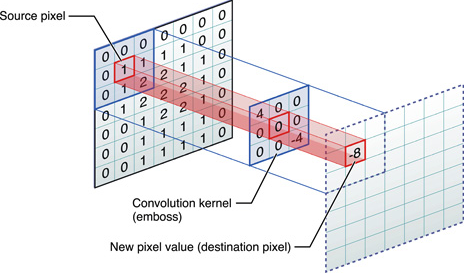
\includegraphics[width=0.5\textwidth]{gfx/kernel}
  \end{center}
  \caption{Convolutional kernel \cite{Apple}.
    The kernel gets centered on the source pixel and the convolution takes into account nearby pixels transforming the source pixel value.
    The convolution operation is a weighted sum of the source pixel with its nearby pixels. In this case:\\
    $(0\cdot4)+(0\cdot0)+(0\cdot0)
     +(0\cdot0)+(1\cdot0)+(1\cdot0)
     +(0\cdot0)+(1\cdot0)+(2\cdot-4) = -8$
  }
  \label{fig:sec:theory:covnets:kernel}
\end{figure}

\begin{figure}[htb]
  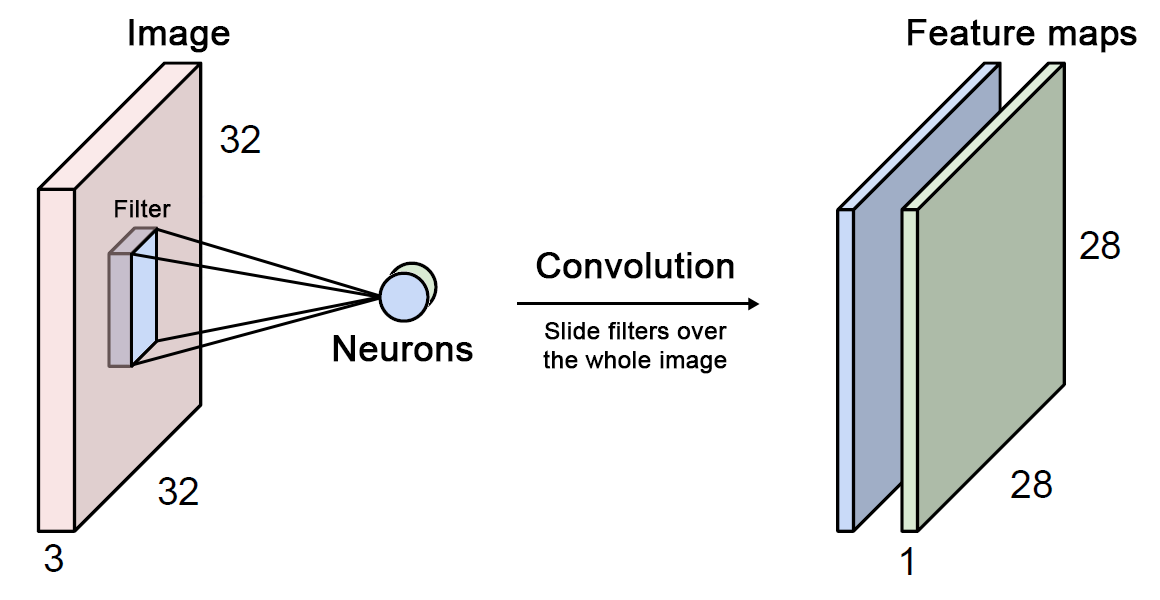
\includegraphics[width=\textwidth]{gfx/conv-layer-2}
  \caption{Anatomy of a convolutional layer and its output \cite{Guerzhoy2016}.
    On the left, there is the representation of an image of ${32}\times{32}$ pixels with $3$ channels (\emph{RGB}).
    Neurons apply a filter of size ${5}\times{5}\times{3}$ in a particular region of the image.
    Neurons of the same color belong to the same slice apply the same filter in different regions of the image and produce a feature map.
    All feature maps combined become the ``new image'' of size ${28}\times{28}\times{N}$, being $N$ the number of slices in the layer, that gets fed to the next layer.}
  \label{fig:sec:theory:conv-layer-2}
\end{figure}

\paragraph{Subsampling}
In the process of detecting higher-order features throughout subsequent layers of the network, the exact absolute position of detected features in feature maps is pretty much irrelevant compared to the relative position between them.
For instance, the pattern that describes the number $7$ is an endpoint in upper left area of a horizontal segment, a corner in the upper right area and an endpoint at the bottom of a vertical segment.
Still, small variations in the input may cause the pattern not to be detected because the features will not completely match the filter.
To make the network more robust against variations the sensitivity of the convolutional layers has to be reduced.
This is effectively accomplished by reducing the resolution of the feature maps through non-linear \emph{subsampling} with pooling layers.
$Max$ is normally used as the non-linear function, giving the name of the subsampling operation \emph{max-pooling}, but it is not limited to it, as we will see in Chapter~\ref{sec:system}.
A pooling layer takes as input a volume of feature maps and, usually, has a non-overlapping filter of size ${2}\times{2}$ that gets applied on each one of the feature maps individually, as can be appreciated in Figure~\ref{fig:sec:theory:convnets:pooling}.
More specifically, the filter summarizes the feature map by performing max-pooling over its ${2}\times{2}$ regions and producing a single value for each, being this a size reduction of $75\%$.
It is important to note that this reduction applies only to the height and width of the original input since the depth refers to the number of feature maps and these are preserved.

\begin{figure}
  \begin{subfigure}[b]{0.35\textwidth}
    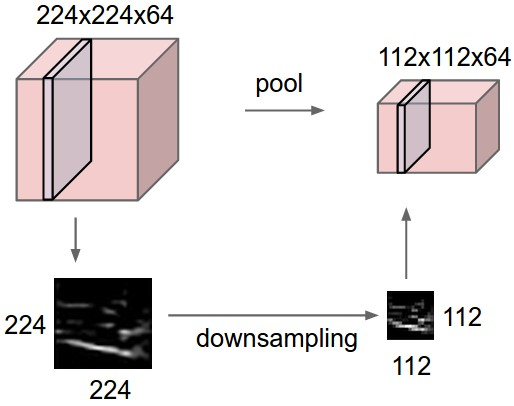
\includegraphics[width=\textwidth]{gfx/pool}
    \captionsetup{justification=centering}
    \caption{General pooling}
    \label{fig:sec:theory:convnets:pooling:general}
  \end{subfigure}
  \hfill
  \begin{subfigure}[b]{0.55\textwidth}
    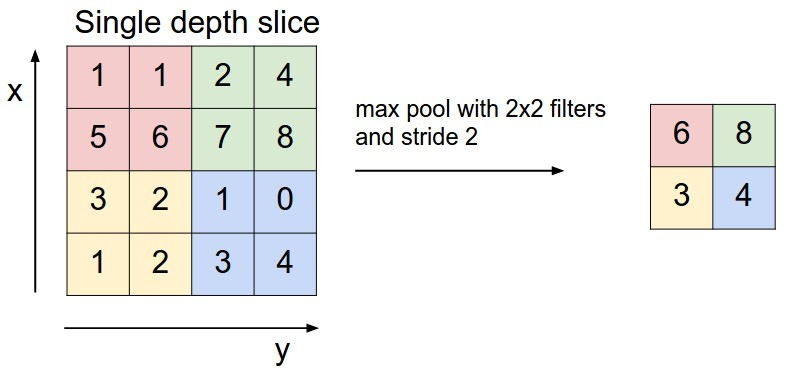
\includegraphics[width=\textwidth]{gfx/maxpool}
    \captionsetup{justification=centering}
    \caption{Max-pooling}
    \label{fig:sec:theory:convnets:pooling:max}
  \end{subfigure}
  \caption{Overview of a pooling layer.
    On the left, the input and output of a pooling layer reducing only the height and width of the volume \cite{Karpathy}.
    On the right, a single feature map of the input volume being subsampled by non-overlapping ${2}\times{2}$ max-pooling \cite{Karpathya}.}
  \label{fig:sec:theory:convnets:pooling}
\end{figure}


\subsection{Architecture}
\label{sub:theory:convnets:achitecture}

While discussing the properties of ConvNets I have introduced two of their building blocks: convolutional layers and pooling layers.
These alone are not enough to use ConvNets for object recognition tasks since feature extraction is not the same as classification.
Let us have a look at how they fit in the big picture and the rest of the building blocks.

In Figure~\ref{fig:sec:theory:convnet} I present the typical configuration of a complete convolutional network.
We can see convolutional layers are alternated with pooling layers and ultimately fed into a fully connected network
Whereas convolutional layers typically increase the amount of feature maps making intermediate representations richer, pooling layers reduce their spatial resolution keeping the amount of parameters low and thus limiting overfitting.
After several convolutional-pooling layers, one final step is a fully connected layer, where the classification takes finally place.
Optionally, normalization layers can be present after convolutional layers to increase the learning rate of the network.
During the learning process, the fully connected layers will be connected to a loss layer that calculates the error of the prediction over a training sample.

\begin{figure}[htb]
  \begin{center}
    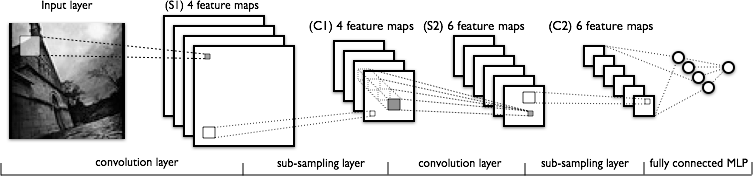
\includegraphics[width=\textwidth]{gfx/conv-network}
  \end{center}
  \caption{LeNet typical architecture \cite{Lisa2010}.
    On the left, there is an image (input layer).
    The image gets processed by a convolutional layer that extracts 4 elementary features producing 4 feature maps (S1).
    A pooling layer reduces the dimensionality while maintaining the same amount of feature maps (C1).
    Next, another convolutional layer extracts 6 higher-order features from the 4 feature maps (C2).
    Again, another pooling layer reduces the resolution of the 6 feature maps (S2).
    Finally, a fully-connected network takes the 6 feature maps and performs classification over them.}
  \label{fig:sec:theory:convnet}
\end{figure}

\paragraph{Fully connected layers}
The fully connected layer is essentially an MLP only that we feed it with the set feature maps produced by the convolutional layers.
Classification is performed in the same fashion as we saw in \autoref{sec:theory:mlp:backpropagation}, but feature maps at that point are a highly abstracted and rich representation of the original image.
That means the data is much less noisy than raw pixels, so overfitting happens to a much lesser degree than what we discussed in \autoref{sec:theory:mlp:overfitting}.

\paragraph{Loss layer}
The loss layer is just a step where the network evaluates the prediction accuracy over ground truth during supervised learning.
In CNNs, a $softmax$ function, defined as the average cross-entropy loss, is normally used.

\paragraph{Normalization layers}
Additionally to these fundamental layers, normalization layers have been used as well, commonly referred to as \emph{Rectified Linear Units} or just \emph{ReLU}.
They simply use non-saturating activation functions like $max$ where the range is $[0,\infty]$, opposed to saturating activation functions like sigmoid where range $[0,1]$ to speed up the training phase \cite{Krizhevsky2012,Nair2010}.
The idea behind using non-saturating activation functions is minimizing the effects of the \emph{vanishing gradient problem} \cite{Socher2015}.
The vanishing gradient problem is a phenomenon in backpropagation that happens when weights adjust too slow on the first layers of very deep networks.
In them, the error contribution of each neuron in the initial layers will be very low and the saturating functions limit unnecessarily how much the weight can be adjusted.
Normalization layers, however, are falling out of use since it has been proved their contribution to the final result is very small and introduces new problems \cite{Lo2015}.

Summarizing, CNNs are mainly composed of convolutional layers, pooling layers, normalization layers, fully connected layers and a loss layer.
Convolutional layers detect features in the input.
Pooling layers reduce the dimensionality of feature maps produced by convolutional layers.
Optionally, normalization layers magnify the non-linear properties of data to speed up learning.
Fully connected layers perform classification like we saw for MLP.
Finally, the loss layer evaluates the quality of the prediction during the training process.


\subsection{Hyperparameters}
\label{sub:theory:convnets:achitecture}

In the next chapters, we will be looking at some already trained ConvNets for image recognition.
Before we move on here is a quick recap of architectural parameters that we will be talking about.

\paragraph{Convolutional input}
The shape of the receptive field in a convolutional layer.
It determines the local connectivity of neurons of the layer with neurons of the previous one.
It is normally larger in the first layer and it decreases for subsequent ones as the resolution decreases.
In image recognition tasks it is common to range from $12x12$ to $15x15$ in the first layer.

\paragraph{Convolutional output}
The spatial arrangement of the output volume from a convolutional layer, which comes defined by \emph{depth}, \emph{stride}, and \emph{zero-padding}.
Depth represents how many neurons are connected to the same receptive field, each one applying a different filter.
It represents how many feature maps are produced as seen in \autoref{fig:sec:theory:convnets:conv-layer-1}.
Looking again at how convolution actually happens in \autoref{fig:sec:theory:covnets:kernel} will help to understand stride and zero-padding.
Stride defines how many units of separation the receptive field moves in the convolution operation and it represents the neuron density loss with respect to the previous layer.
With stride 1 there will be no ``gaps'' between neurons and their receptive field will be highly overlapped.
As stride goes up more ``gaps'' will appear, reducing the resolution of the output and making neurons' receptive field less overlapped.
Lastly, as seen in the convolution operation, the resolution of the result is smaller than the original on the edges.
Zero-padding is used to pad the output volume with zeros when maintaining the same resolution is required.

\paragraph{Pooling filter}
Shape of the filter in pooling layers, defined by height, width, and stride.
Usually $2x2$ filter with stride 2 are used, as in the example depicted in \autoref{fig:sec:theory:convnets:pooling:max}.
Stride is set to 2 so that the filters do not overlap.

\todo[inline]{Maybe talk about regularization methods? Dropout?}
